\documentclass[11pt]{beamer}
\usepackage[T1]{fontenc}
\usepackage{hyperref}
\usepackage{url}
\usepackage{xcolor}
\usepackage[linesnumbered, ruled, longend]{algorithm2e}
\usepackage{colortbl}
\usepackage{subcaption}
\usepackage{amsmath,amssymb}
\usepackage{ragged2e}
\usepackage{multirow}
\usepackage{changepage}
\setbeamerfont{frametitle}{size=\large}
\usepackage{caption}
\captionsetup{labelformat=empty}
\usepackage{booktabs}
\usepackage{array}
\newcolumntype{P}{>{\centering\arraybackslash}p}
%\usepackage{enumitem}
% \usepackage[table,xcdraw]{xcolor}
% \usepackage{etoolbox}
\renewcommand{\raggedright}{\leftskip=0pt \rightskip=0pt plus 0cm}
\apptocmd{\frame}{}{\justifying}{}
\let\oldenumerate=\enumerate 
\renewenvironment{enumerate}{\oldenumerate\raggedright}{\endlist} 
\let\olditemize=\itemize
\renewenvironment{itemize}{\olditemize\raggedright}{\endlist}

\usepackage{xcolor}
\definecolor{commentgreen}{RGB}{2,112,10}
\definecolor{eminence}{RGB}{108,48,130}
\definecolor{weborange}{RGB}{255,165,0}
\definecolor{frenchplum}{RGB}{129,20,83}

\usepackage{listings}
\usepackage{textcomp}
\lstset {
	language=Java,
	frame=tb,
	tabsize=4,
	showstringspaces=false,
	numbers=left,
	upquote=true,
	commentstyle=\color{commentgreen},
	keywordstyle=\color{eminence},
	stringstyle=\color{red},
	basicstyle=\small\ttfamily, % basic font setting
	emph={int,char,double,float,unsigned,void,bool},
	emphstyle={\color{blue}},
	escapechar=\&,
	% keyword highlighting
	classoffset=1, % starting new class
	morekeywords={>,<,.,;,,,-,!,=,~},
	keywordstyle=\color{weborange},
	classoffset=0,
}

\usepackage{adjustbox}
\newcommand{\code}[1]{\texttt{#1}}

\usetheme{Warsaw}
\useoutertheme{smoothtree}
\usepackage[utf8]{vietnam}
%%%%%%%%%%%%%%%%%%%%%%%%%%%%%%%%%%%%
\def\mydate{\leavevmode\hbox{\bfseries\the\day/\twodigits\month/\twodigits\year}}
\def\twodigits#1{\ifnum#1<10 0\fi\the#1}
%%%%%%%%%%%%%%%%%%%%%%%%%%%%%%%%%%%%
\definecolor{sectioncolor}{RGB}{39,0,118}
\definecolor{framecolor}{RGB}{37,109,255}

\setbeamercolor{frametitle}{fg=white, bg=blue}
\definecolor{light-gray}{gray}{0.95}
%%%%%%%%%%%%%%%%%%%%%%%%%%%%%%%%%%%
\setbeamertemplate{footline}
{%
	\leavevmode%
	\begin{beamercolorbox}[wd=.5\paperwidth,ht=2.75ex,dp=1.5ex]{author in head/foot}%
		\hbox to .5\paperwidth{\hfil\insertshortauthor\hfil}
	\end{beamercolorbox}%
	\begin{beamercolorbox}[wd=.5\paperwidth,ht=2.75ex,dp=1.5ex]{date in head/foot}%
		\raggedleft
		\usebeamerfont{date in head/foot}
		\insertframenumber{} / \inserttotalframenumber\hspace*{15pt}
	\end{beamercolorbox}%
}
%==============================================
\makeatletter
\patchcmd{\beamer@sectionintoc}
{\vfill}
{\vskip\itemsep}
{}
{}
\makeatother  
\begin{document}
\captionsenglish
\dateUSenglish
\author[Le Vu Loi]{
	\begin{center}
		{\fontsize{14pt}{\baselineskip}\selectfont Le Vu Loi - 20173240} \\[10pt]
		{\fontsize{12pt}{\baselineskip}\selectfont Talented class of Computer Science} \\[25pt]
		\textbf{Supervisor}: Assoc. Prof. Pham Van Hai\\
		Department of Information System
	\end{center}
%	\begin{tabular}{ll}
%		Le Vu Loi - 20173240 \\[]
%		
%		\textit{Supervisor} & Assoc. Prof. Pham Van Hai
%	\end{tabular}
}
\title[]{\bfseries\fontsize{14}{\baselineskip}\selectfont BACHELOR THESIS\vspace{5pt}}
\subtitle{The proposed Dual Encoder model for Open-domain
	question answering system: Case study in Vietnamese
	COVID-19 topic}
\logo{
\includegraphics[scale=.1]{images/SoICTlogo.jpg}}
\institute[\bfseries Viện CNTT\&TT]{}
\date[\mydate]{\today}
%\subject{Yo!}

\begin{frame}[plain]
	\maketitle
\end{frame}
%====================================
\begin{frame}[plain]
\frametitle{Outline}
\begin{columns}[t]
	\begin{column}{.5\textwidth}
		\tableofcontents[sections={1-3}]
	\end{column}
	\begin{column}{.5\textwidth}
		\tableofcontents[sections={4-6}]
	\end{column}
\end{columns}
\end{frame}
%====================================
\section{Introduction}
\subsection{Overview}
\begin{frame}
\frametitle{Open-domain question answering}
\hspace*{-15pt}
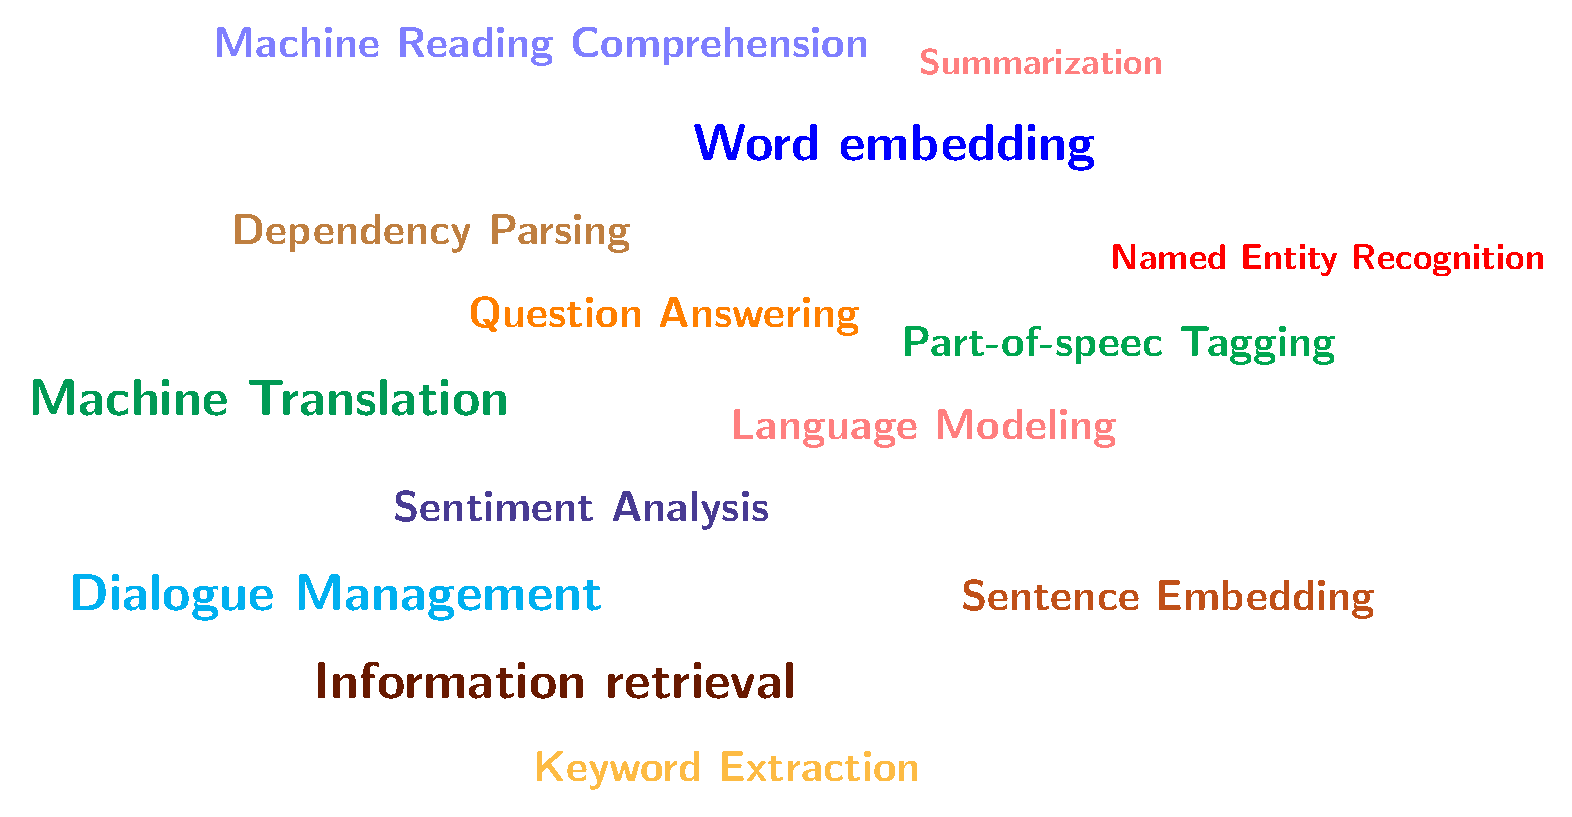
\includegraphics[scale=.45]{images/PDF/nlptask/nlptask.pdf}
\end{frame}
%====================================
%\begin{frame}
%\frametitle{Open-domain question answering}
%\textbf{Open-domain question answering is at medium level of difficulty among various NLP tasks.} \\[10pt]
%\begin{itemize}
%\item Word embedding
%\item Sentence embedding
%\item Language Modeling \\
%.....
%\item Question Answering
%\item \textcolor{blue}{\bfseries Open-domain question answering}\\
%.....
%\item Text Summarization
%\item Dialogue Management
%\end{itemize}
%\end{frame}
%====================================
\begin{frame}
\frametitle{Open-domain question answering}
%\vspace{-.5cm}
\begin{itemize}
	\item Combination of \textbf{retriever} (Information Retrieval) and \textbf{reader} (Machine Reading Comprehension)
	\begin{itemize}
		\item "Skim through" a large data source to find a subset of relevant documents.
		\item "Swallow" each document to find the exact answer(s).
	\end{itemize}
\end{itemize}
%\hspace*{-15pt}
%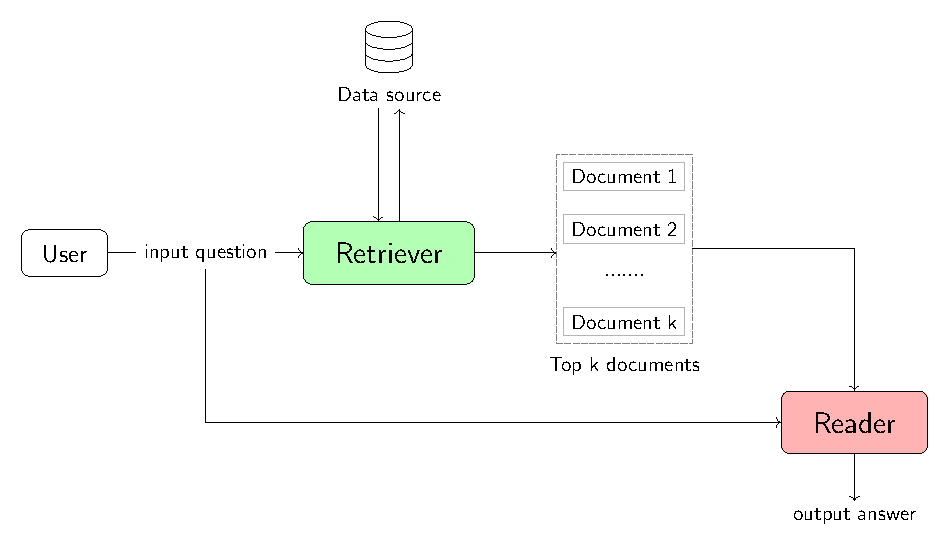
\includegraphics[scale=.68]{images/PDF/overall_arch/architecture.pdf}
\end{frame}
%====================================
\subsection{Problem formulation}
\begin{frame}
\begin{adjustwidth}{-2em}{1em}
\frametitle{Problem formulation}
\begin{itemize}
	\item \textbf{Input} 
	\begin{itemize}
		\item A question in human natural language.\\[5pt]
		\textit{E.g.} Who is the founder of Google?
	\end{itemize}
	\item \textbf{Output}
	\begin{itemize}
		\item A list of answers for the input question \\[5pt]
		\textit{E.g.} [Larry Page, Sergey Brin]
	\end{itemize}
	\item \textbf{Constraints}
	\begin{itemize}
		\item The system answers only factoid question.
%		\item Factoid question means that the question is about a fact and often can be answered by a short phrase. Yes/no question, multiple-choice question and reasoning question are not factoid. \\[5pt]
%		- \textit{Factoid question}: What is the capital of Vietnam? \\
%		- \textit{Reasoning question}: If 3 cats can catch 3 mice in 3 minutes, how many mices can 6 cats catch in 6 minutes?
	\end{itemize}
%\begin{figure}
%	content...
%\end{figure}
\end{itemize}
\end{adjustwidth}
\end{frame}
%====================================
\section{Related works}
\begin{frame}
\frametitle{Related works}
\begin{thebibliography}{10}
	\bibitem{mrc}
	[1] Danqi Chen, Adam Fisch, Jason Weston, and Antoine Bordes. Reading wikipedia to answer open-domain questions. \underline{arXiv preprint arXiv:1704.00051}, 2017.
	\bibitem{dpr}
	[2] Vladimir Karpukhin, Barlas Oguz, Sewon Min, Patrick Lewis, Ledell Wu, Sergey Edunov, Danqi Chen, and Wen-tau Yih. Dense passage retrieval for open-domain	question answering. \underline{arXiv preprint arXiv:2004.04906}, 2020.
\end{thebibliography}
\end{frame}
%====================================
\begin{frame}
\frametitle{Reading Wikipedia to answer open-domain questions}
\begin{itemize}
%	\item Danqi Chen et. al \cite{mrc} proposed to solve open-domain question answering problem by reading Wikipedia to find answers.
%	\item Consist of a \textbf{document retriever} based on bigram hashing and TF-IDF matching and \textbf{machine reader} based on multi-layer Recurrent neural network.Chen et. al \cite{mrc} proposed to solve open-domain question answering problem by reading Wikipedia to find answers.
%\item Consist of a \textbf{document retriever} based on bigram hashing and TF-IDF matching and \textbf{machine reader} based on multi-layer Recurrent neural network.
%\item This work promoted a large number of subsequent publications on Open-domain question answering problem.
%	\item This work promoted a large number of subsequent publications on Open-domain question answering problem.
	\item \textbf{Retriever}: bigram hashing and TF-IDF matching
	\item \textbf{Reader}: Multi-layer recurrent neural network
	\item Potential improvements: using neural network to better capture documents' semantics
\end{itemize}
\end{frame}
%====================================
\begin{frame}
\frametitle{Dense passage retrieval}
\begin{itemize}
%	\item Karpukhin et. al \cite{dpr} proposed to use a dense retriever which based on Dual encoder architecture for retrieving documents in open-domain question answering system.
%	\item Dual encoder consists of a question encoder and a context encoder, which is used to encode question and document respectively into (a) vector space(s).
%	\item Similarity between a document and a question is computed by taking dot product of the encoded question and the encoded document.
%	\item Relevant documents to the input question are retrieved using this similarity.
	\item \textbf{Retriever}: Dual-encoder
	\item \textbf{Reader}: Cross-encoder
	\item Successfully use neural network to solve information retrieval.
	\item Potential improvements: More challenging learning task for the system to gain deeper language understanding.
\end{itemize}
\end{frame}
%====================================
\section{Proposed method}
\subsection{System pipeline}
\begin{frame}
\frametitle{System pipeline}
\begin{itemize}
	\item Open-domain question answering = Retriever + Reader
\end{itemize}
\hspace*{-15pt}
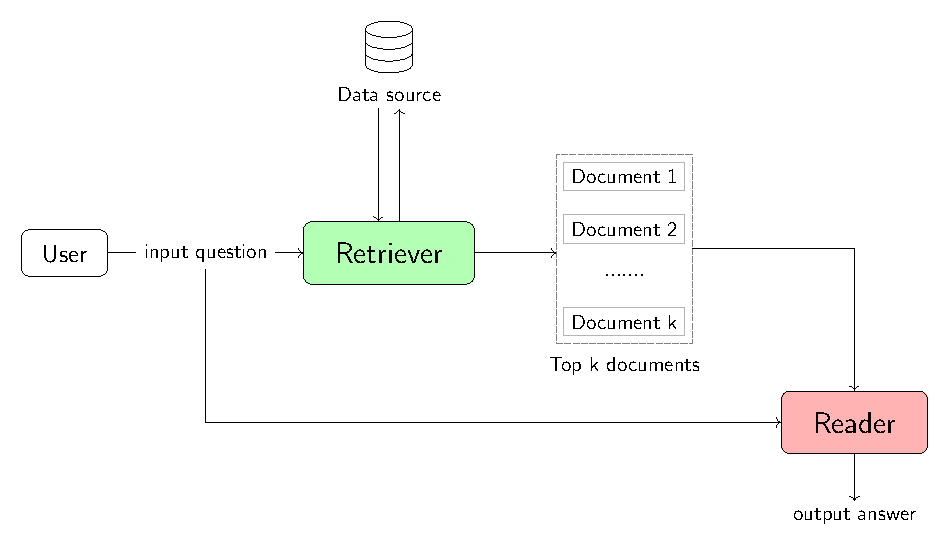
\includegraphics[scale=.68]{images/PDF/overall_arch/architecture.pdf}
\end{frame}
%====================================
\subsection{Retriever}
\begin{frame}
	\frametitle{Dense retriever: Dual encoder architecture}
	\begin{itemize}
		\item Dense retriever is based on Dual encoder architecture.
	\end{itemize}
	\begin{figure}[h]
		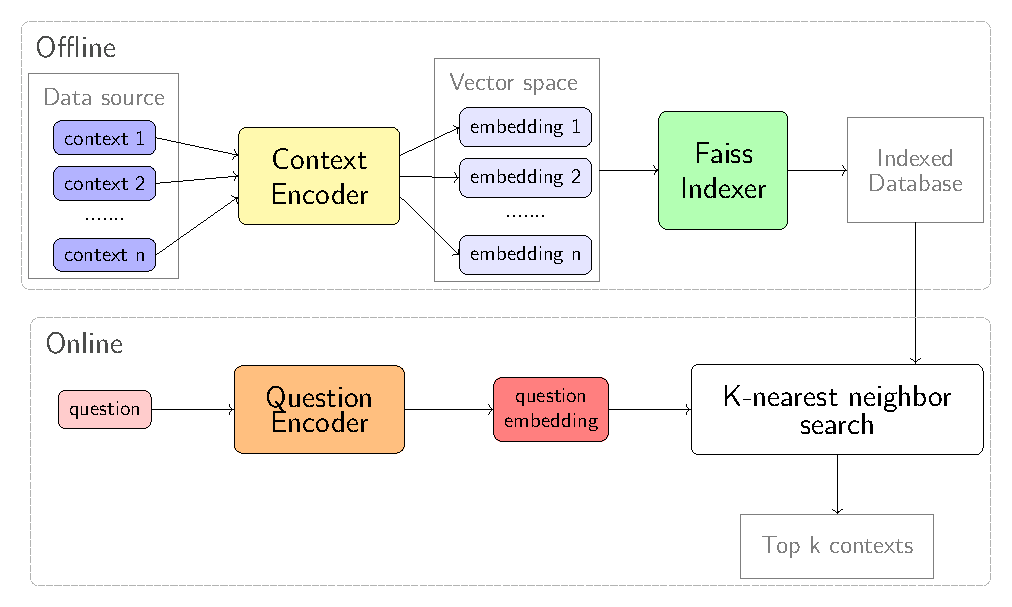
\includegraphics[scale=.57]{images/PDF/biencoder/biencoder.pdf}
		\caption{Workflow of a dense retriever}
	\end{figure}
\end{frame}
%====================================
\begin{frame}
\frametitle{Training dense retriever}
\begin{itemize}
	\item Jointly train question encoder and context encoder.
	\item Training data: a training sample consists of:
	\begin{itemize}
		\item $q$: input question.
		\item $p^+$: positive context, which is the document that contains the answers.\\[5pt]
		\item $\left\{p^-_j\right\}_{j=1}^m$: $m$ negative contexts, which are documents that do not contain the answers.
	\end{itemize}
	\item Loss function (per one training sample): negative log-likelihood
	\begin{equation}
		\label{eq:01}
		\mathcal{L} = -\log\left\{\dfrac{\exp\left[{\text{sim}\left(q, p^+\right)}\right]}{\exp\left[{\text{sim}\left(q, p^+\right)}\right] + \sum\limits_{j=1}^m \exp\left[{\text{sim}\left(q, p^-_j\right)}\right]}\right\}
	\end{equation}
\end{itemize}
\end{frame}
%====================================
\subsection{Reader}
\begin{frame}
	\frametitle{Extractive reader: Cross encoder architecture}
	\begin{itemize}
		\item Extractive reader's task is to predict the start and end position of answer in the documents returned by dense retriever.\\
		\begin{center}
		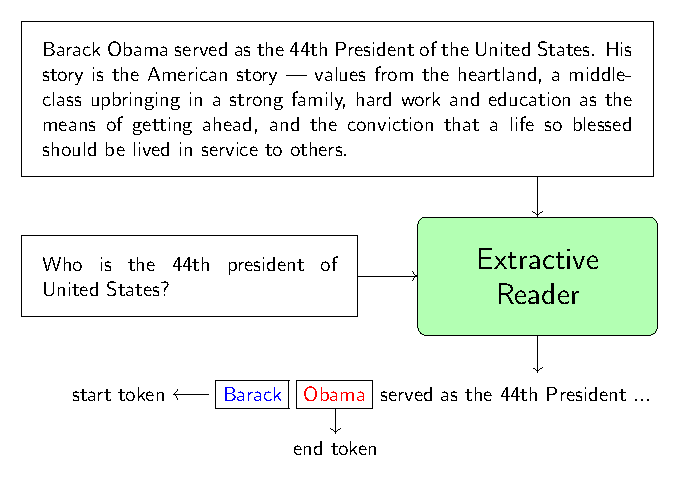
\includegraphics[scale=.55]{images/PDF/extractive_reader/extractive_reader.pdf}
		\end{center}
		\item Extractive reader consists of 2 components, in which each component follows a cross encoder architecture:
		\begin{itemize}
			\item Re-ranker: re-rank documents returned by dense retriever.
			\item Single-document reader: read one document to extract answers.
		\end{itemize}
	\end{itemize}
\end{frame}
%====================================
\begin{frame}
\frametitle{Re-ranker}
\vspace*{-20pt}
\begin{figure}[h]
	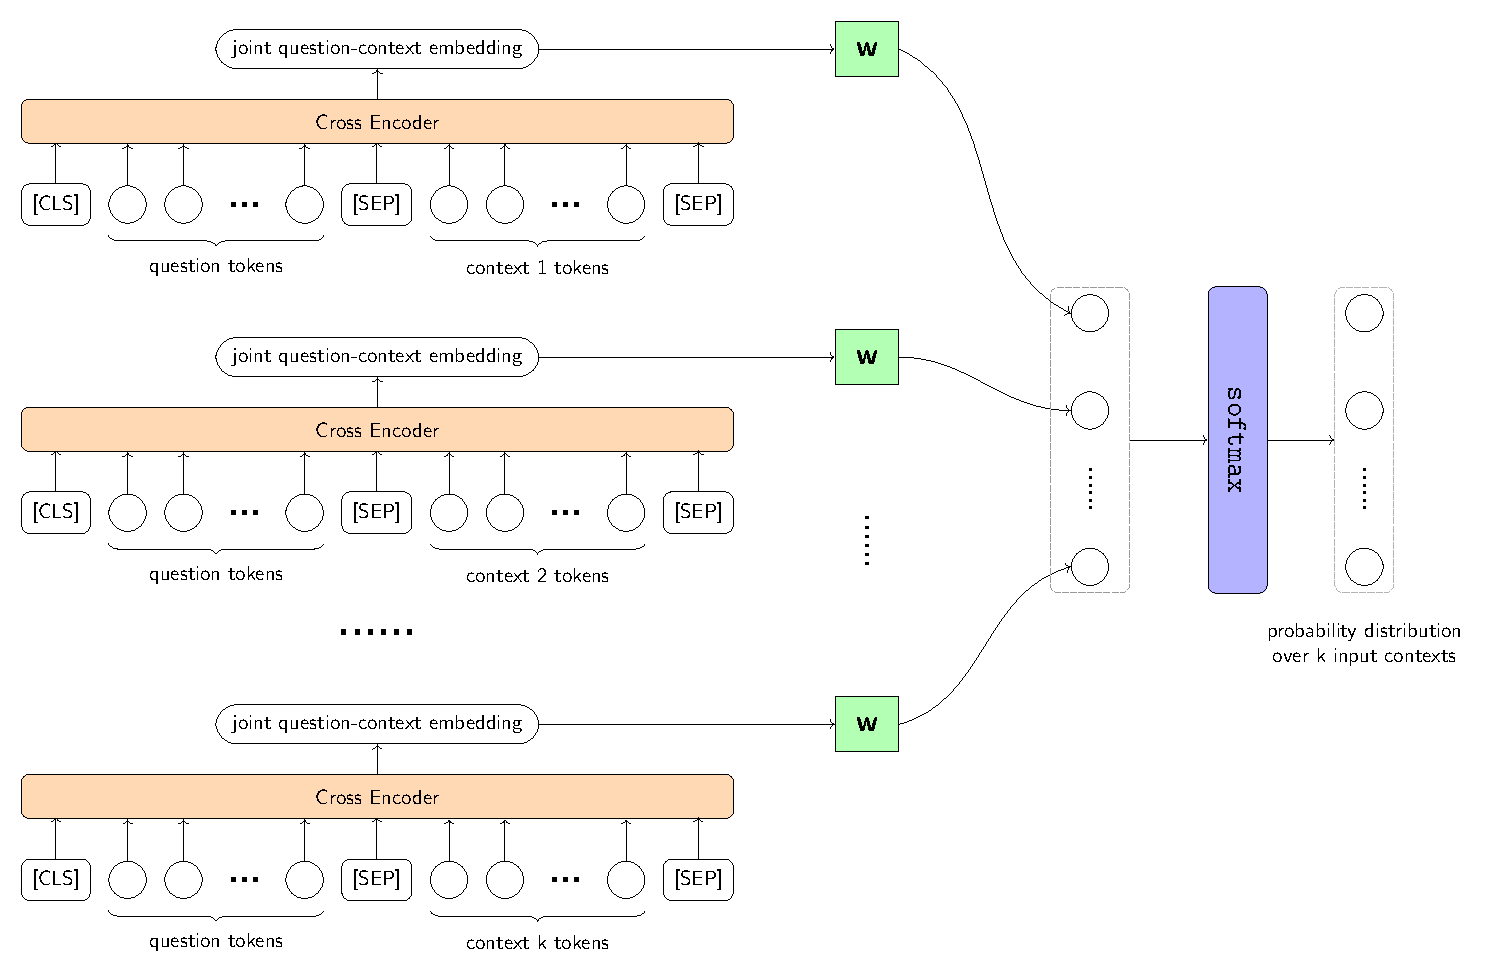
\includegraphics[scale=.43]{images/PDF/full-reranker/fullRerank.pdf}
	\caption{Model architecture}
\end{figure}
\end{frame}
%====================================
%\begin{frame}
%\frametitle{Training re-ranker}
%\begin{adjustwidth}{-2em}{0em}
%\begin{itemize}
%	\item {\fontsize{10pt}{\baselineskip}\selectfont Target to maximize probability of positive context over negative contexts.}
%	\item {\fontsize{10pt}{\baselineskip}\selectfont Training data: a training sample consists of:}
%	\begin{itemize}
%		\item {\fontsize{9pt}{\baselineskip}\selectfont$q$: input question.}
%		\item {\fontsize{9pt}{\baselineskip}\selectfont$p^+$: positive context.}
%		\item {\fontsize{9pt}{\baselineskip}\selectfont$\left\{p_j^-\right\}_{j=1}^m$: $m$ negative contexts.}
%	\end{itemize}
%	\item {\fontsize{10pt}{\baselineskip}\selectfont Loss function}
%	\begin{itemize}
%		\item {\fontsize{9pt}{\baselineskip}\selectfont Assumptions}
%		\begin{itemize}
%			\item {\fontsize{8pt}{\baselineskip}\selectfont$e^+$: joint question-context embedding vector of input question and positive context.}
%			\item {\fontsize{8pt}{\baselineskip}\selectfont$\left\{e_j^-\right\}_{j=1}^m$: $m$ joint question-context embedding vectors of input question and negative contexts.}
%		\end{itemize}
%	\item {\fontsize{9pt}{\baselineskip}\selectfont Loss formula}
%	\begin{scriptsize}
%	\begin{equation}
%		\label{eq:02}
%		\mathcal{L} = -\log\left\{\dfrac{\exp\left(e^+\mathbf{w}\right)}{\exp\left(e^+\mathbf{w}\right) + \sum\limits_{j=1}^m\exp\left(e_j^-\mathbf{w}\right)}\right\}
%	\end{equation}
%	where $w$ is a learnable vector.
%	\end{scriptsize}
%	\end{itemize}
%\end{itemize}
%\end{adjustwidth}
%\end{frame}
%====================================
\begin{frame}
\frametitle{Single-document reader}
\vspace*{-10pt}
\begin{figure}[h]
	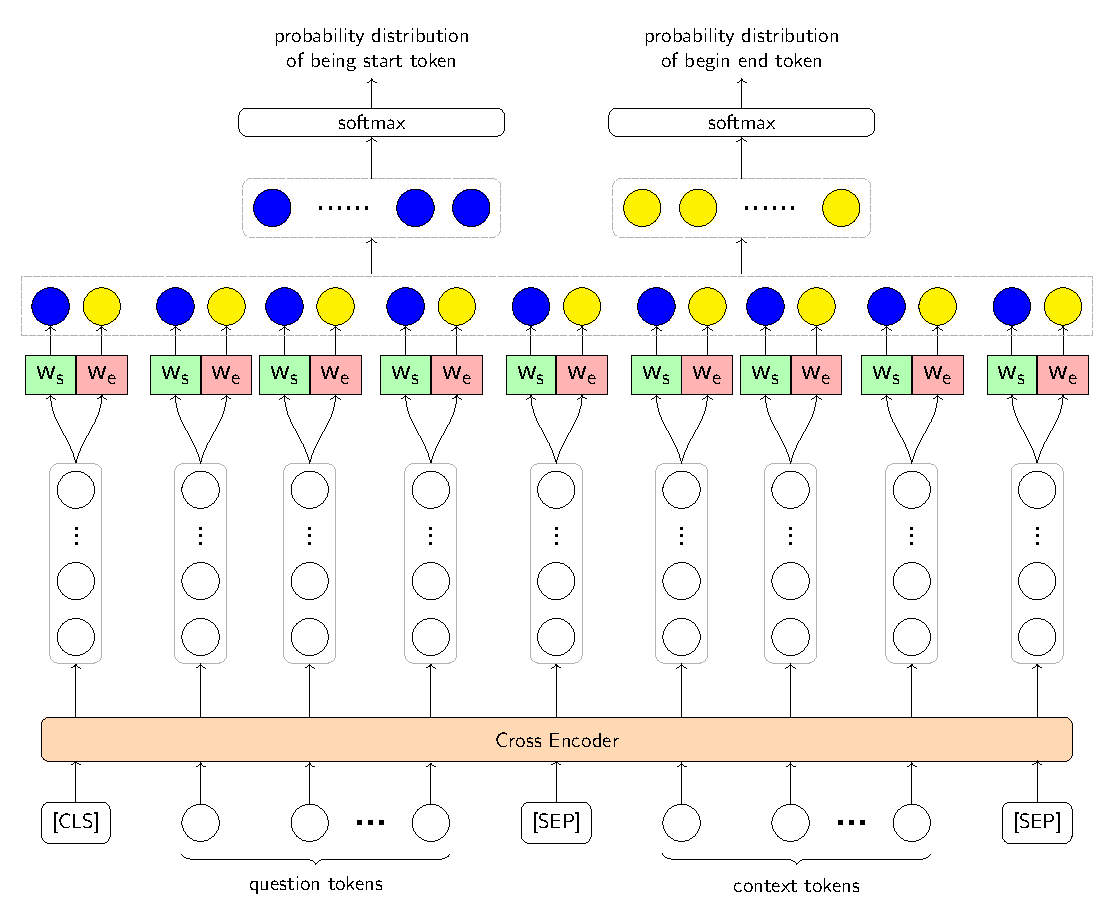
\includegraphics[scale=.45]{images/PDF/singleDocReader/singleDocReader.pdf}
	\caption{Model architecture}
\end{figure}
\end{frame}
%====================================
%\begin{frame}
%\frametitle{Training single-document reader}
%%\begin{adjustwidth}{-2em}{0em}
%\begin{itemize}
%	\item {\fontsize{10pt}{\baselineskip}\selectfont Target to maximize joint probability of answer's start and end position.}
%	\item {\fontsize{10pt}{\baselineskip}\selectfont Training data: a training sample consists of:}
%	\begin{itemize}
%		\item $L$: concatenation of input question and a positive context.
%		\item $s$: start position of the answer.
%		\item $e$: end position of the answer.
%	\end{itemize}
%	\item {\fontsize{10pt}{\baselineskip}\selectfont Loss function}
%	\begin{itemize}
%		\item Assumptions
%		\begin{itemize}
%%			\item $h$: joint question-context embedding vector.
%			\item $\alpha$: probability distribution of being start position.
%			\item $\beta$: probability distribution of being end position.
%		\end{itemize}
%		\item Loss function
%		\begin{equation}
%			\label{eq:03}
%			\mathcal{L} = -\log{\alpha[s]} -\log{\beta[e]}
%		\end{equation}
%	\end{itemize}
%\end{itemize}
%%\end{adjustwidth}
%\end{frame}
%====================================
\subsection{Stratified loss}
%\begin{frame}
%\frametitle{Existing approach: in-batch loss}
%\begin{adjustwidth}{-2em}{0em}
%\begin{itemize}
%	\item Karpukhin et. al \cite{dpr} proposed to use in-batch strategy and hard negative contexts to train dense retriever using negative log-likelihood loss defined in equation~\eqref{eq:01}. To be specific:
%	\begin{itemize}
%		\item In-batch strategy: training samples in a training batch use others' positive context as their negative contexts \\ $\rightarrow$ significantly reduce the number of documents needed to be fed into context encoder.
%		\item Hard negative contexts: normal negative contexts are non-relevant to the input question. Hard negative contexts are relevant to the input question but do not contain required information to answer that question. \\[5pt]
%		$\rightarrow$ challenge the model to learn better.
%	\end{itemize}
%\end{itemize}
%\end{adjustwidth}
%\end{frame}
%====================================
\begin{frame}
\frametitle{Proposed method: stratified loss for training dual encoder}
\begin{adjustwidth}{-2em}{0em}
\begin{itemize}
	\item Idea: additional loss for learning difference between hard negative and normal negative contexts.
	\item Stratified loss
	\begin{itemize}
		\item Assumptions: a batch of $b$ training samples $\mathcal{D}$, where the $i$-th training sample $\mathcal{D}_i$ consists of:
		\begin{itemize}
			\item $q_i$: input question.
			\item $p_i^+$: positive context.
			\item $\left\{p_{i,j}^-\right\}_{j=1}^m$: $m$ hard negative contexts.
		\end{itemize}
		\item Loss formula
	\end{itemize}
\end{itemize}
\begin{scriptsize}
\begin{equation}
	\label{eq:04}
	\begin{array}{ll}
		\mathcal{L} = &-\log\left\{\dfrac{\exp\left[{\text{sim}\left(q_i, p_i^+\right)}\right]}{\exp\left[{\text{sim}\left(q_i, p_i^+\right)}\right] + \sum\limits_{j=1}^m \exp\left[{\text{sim}\left(q_i, p_{i,j}^-\right)}\right]}\right\} \\[20pt]
		&-\sum\limits_{j=1}^m\log\left\{\dfrac{\exp\left[{\text{sim}\left(q_i, p_{i,j}^-\right)}\right]}{\exp\left[{\text{sim}\left(q_i, p_{i,j}^-\right)}\right] + \sum\limits_{k \in \{1,2,...,b\} \backslash \{i\}}\exp\left[\text{sim}\left(q_i, p_k^+\right)\right]}\right\}
	\end{array}
\end{equation}
\end{scriptsize}
\end{adjustwidth}
\end{frame}
%====================================
\section{Case study}
\begin{frame}
	\frametitle{Case study on Vietnamese COVID-19 topic}
	\begin{itemize}
		\item Building an open-domain question answering for Vietnamese COVID-19 topic requires:
		\begin{itemize}
			\item Building a context source for COVID-19 topic, which contains all documents that the system searches during answering a question about COVID-19 topic.
			\item Annotate data for training dense retriever and extractive reader (re-ranker and single-document reader).
		\end{itemize}
	\end{itemize}
\end{frame}
%====================================
\subsection{Data crawling}
\begin{frame}
\frametitle{Data crawling for COVID-19 data}
\begin{itemize}
\item Context source: 168,388 contexts/documents about medial topic,  mainly crawled from \url{https://suckhoedoisong.vn/}
\item Training data: 995 training samples, in which each sample consists of:
\begin{itemize}
	\item Input question
	\item One positive context
	\item One hard negative context
	\item List of answers
\end{itemize}
\end{itemize}
\end{frame}
%====================================
\subsection{Data annotating}
\begin{frame}
\frametitle{Data annotating}
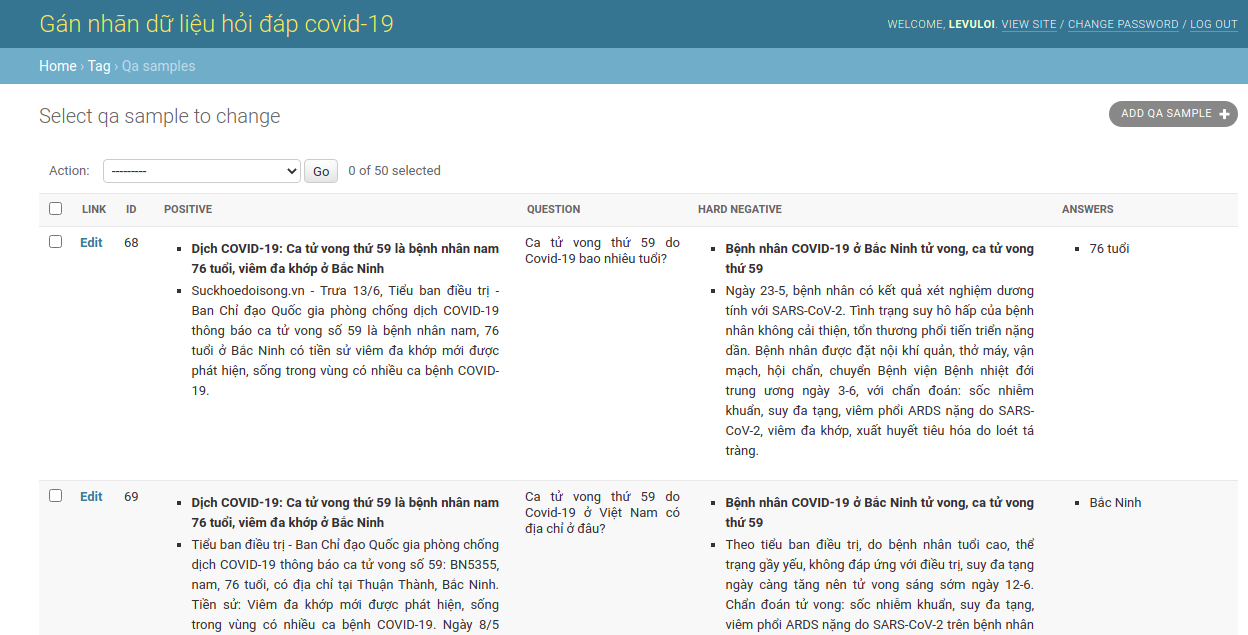
\includegraphics[scale=.25]{images/annotate.png}
\end{frame}
%====================================
%\subsection{Pretrained model}
%\begin{frame}
%	\frametitle{Pretrained model}
%	\begin{adjustwidth}{0em}{5em}
%	\begin{itemize}
%		\item Vietnamese open-domain question answering for COVID-19 topic was trained from the pretrained language model {\tt NlpHUST/vibert4news-base-cased} pulling from \href{https://huggingface.co/}{\tt huggingface}
%		\item Another well-known pretrained language model for Vietnamese is {\tt PhoBERT} of VinAI, which can also be found on \href{https://huggingface.co/}{\tt huggingface}
%	\end{itemize}
%	\end{adjustwidth}
%\end{frame}
%====================================
\section{Experimental results}
\begin{frame}
\frametitle{Datasets}
\begin{itemize}
	\item Google Natural Question: preprocessed data taken from \cite{dpr}
	\begin{itemize}
		\item 58,880 training samples
		\item 8,757 development samples
		\item 3,610 test samples
		\item Context source contains 21,015,324 contexts
		\item To rapidly produce experiments, the context source is reduced to 700,000 contexts and 450 additional contexts are considered to cover all input questions in the test set. 
	\end{itemize}
	\item Vietnamese COVID-19 datatset
	\begin{itemize}
		\item 995 training samples
		\item Context source contains 168,388 contexts
	\end{itemize}
\end{itemize}
\end{frame}
%=======================================
\begin{frame}
\frametitle{Metrics}
\begin{itemize}
	\item Top-$k$ hit scores
	\begin{itemize}
		\item Measure retriever's accuracy
		\item Top-$k$ hit is reached if at least one of $k$ contexts returned by the retriever contains answer(s) for input question. 
	\end{itemize}
	\item Exact match
	\begin{itemize}
		\item Measure reader's accuracy
		\item Measure end-to-end system's accuracy
		\item An exact match hit is reached if answer(s) produced by the open-domain question answering system matches exactly the ground truth answer(s)
	\end{itemize}
\end{itemize}
\end{frame}
%=======================================
\begin{frame}
\frametitle{System settings}
\begin{adjustwidth}{-2em}{0em}
\begin{itemize}
	\item Using Google Cloud Platform
	\item Training and inference on Cloud TPUs
	\item Process data on VM Compute Engine
\end{itemize}
\vspace{1cm}
\begin{table}[!htbp]
\centering
\caption{Hardware configurations}
\begin{tabular}{p{.45\linewidth}p{.45\linewidth}}
	\toprule
	Cloud TPUs & VM Compute Engine \\
	\midrule
	\begin{minipage}{6cm}
		TPU v3-8 on-demand:
		\begin{itemize}
			\item TPU version 3
			\item 8 TPU cores
			\item 16GiB memory / TPU core
		\end{itemize}
	\end{minipage} & \begin{minipage}{6cm}
		\begin{itemize}\item OS: Ubuntu 20.04  \item Disk: 30GB \item RAM: 16GB \item nCPUs: 4\end{itemize}
	\end{minipage} \\
	\bottomrule
\end{tabular}
\end{table}
\end{adjustwidth}
\end{frame}
%=======================================
\begin{frame}
\frametitle{Results on dense retriever}
\begin{adjustwidth}{-2em}{0em}
\begin{itemize}
	\item Experimental results on dense retriever are conducted using Google Natural Question dataset.
	\item The proposed method was compared to the baseline in \cite{dpr}
\end{itemize}
\begin{figure}
\begin{minipage}{.45\linewidth}
%\raggedright
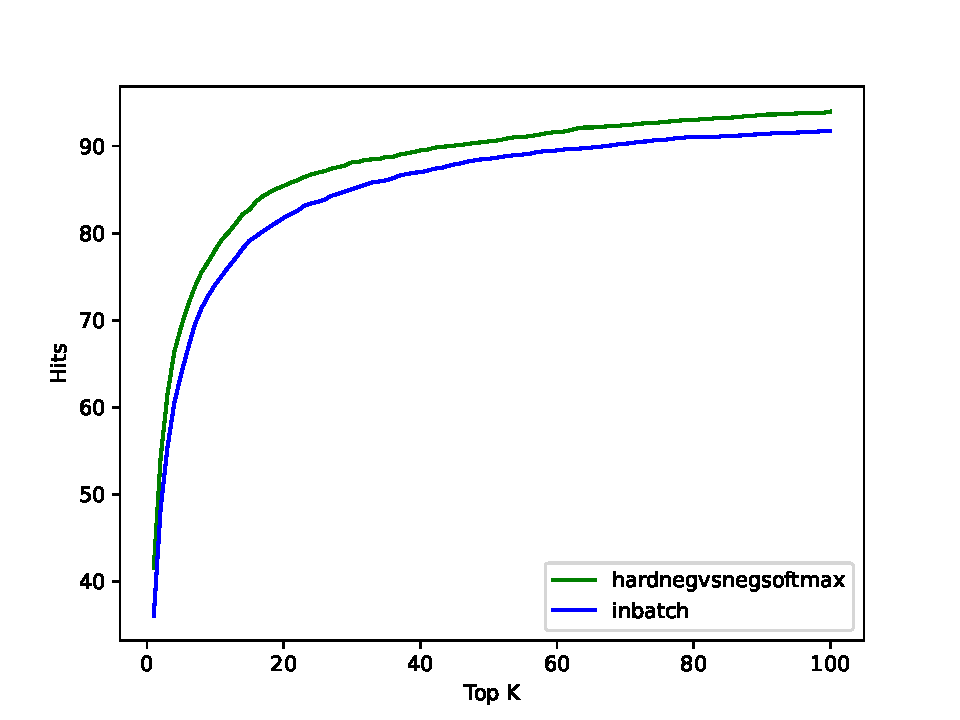
\includegraphics[scale=.32]{images/PDF/experiments/inbatch_hardnegvsnegsoftmax_4-1-5.pdf}
\caption{\fontsize{8pt}{\baselineskip}\selectfont Comparasion results with baseline model implemented}
\end{minipage}
\hfill
\begin{minipage}{.45\linewidth}
\raggedleft
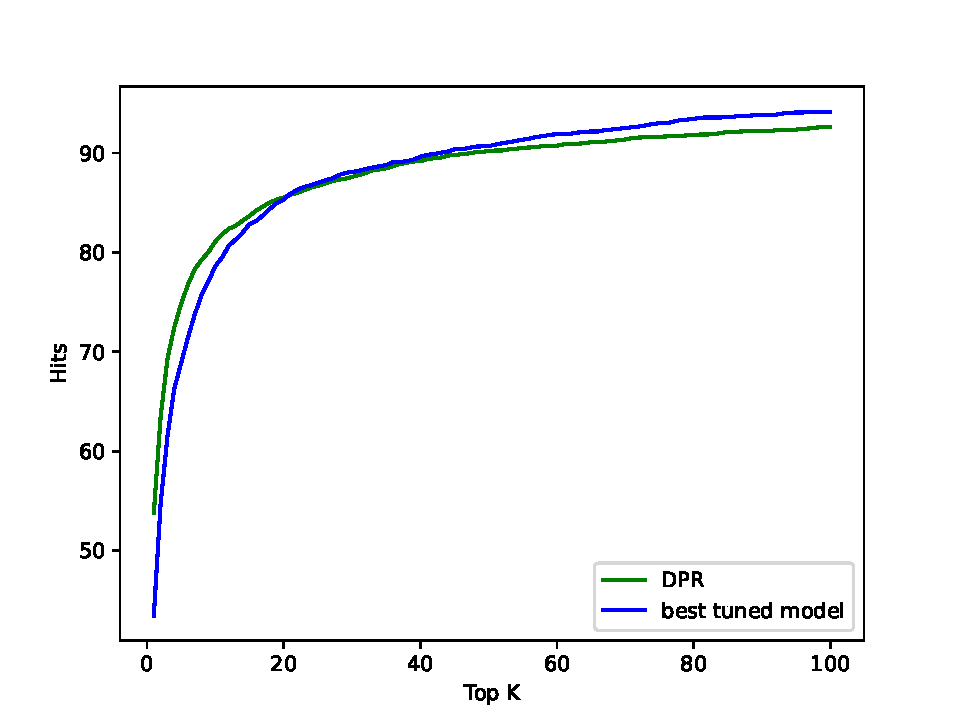
\includegraphics[scale=.32]{images/PDF/experiments/benchmark_compare.pdf}
\caption{\fontsize{8pt}{\baselineskip}\selectfont Comparasion results with baseline model taken from released checkpoint}	
\end{minipage}
\end{figure}
\end{adjustwidth}
\end{frame}
%=======================================
%\begin{frame}
%\frametitle{Results on extractive reader}
%\begin{itemize}
%	\item Experimental results on extractive reader are conducted using Google Natural Question.
%	\item Exact match score: 56.6\%
%\end{itemize}
%\end{frame}
%=======================================
%\subsection{Web demo}
%\begin{frame}
%\frametitle{Question Answering about COVID-19}
%\begin{adjustwidth}{-2em}{-2em}
%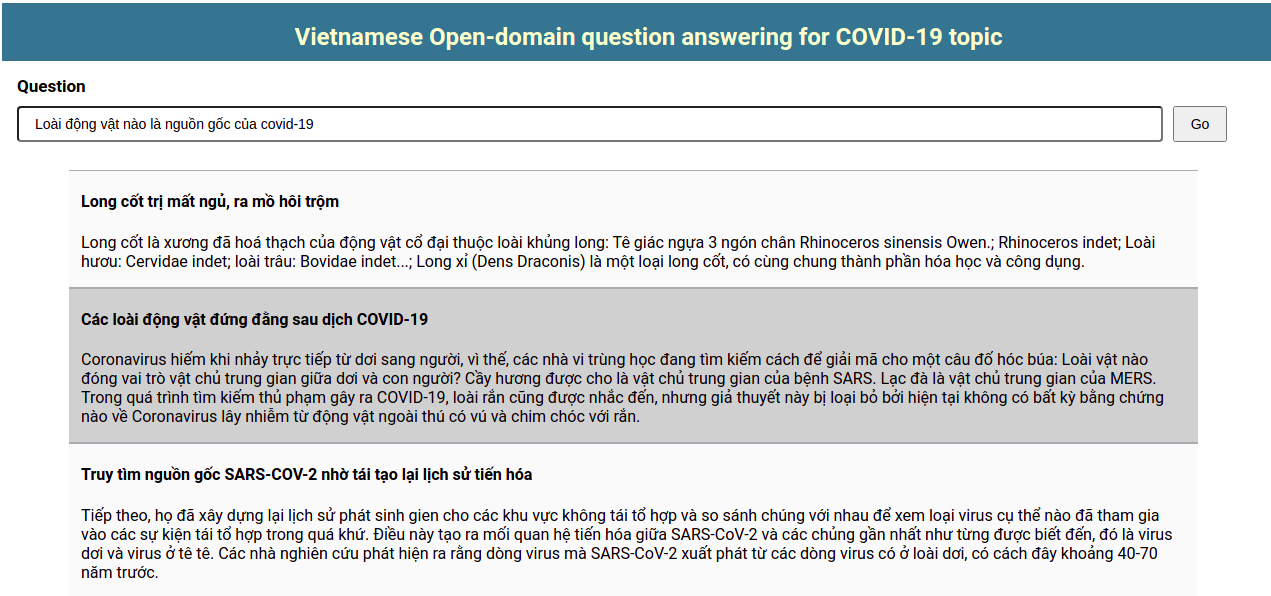
\includegraphics[scale=.27]{images/VNQA.png}
%\end{adjustwidth}
%\end{frame}
%=======================================
\begin{frame}
\frametitle{Demo: Question Answering about COVID-19}
\begin{adjustwidth}{-2em}{-2em}
	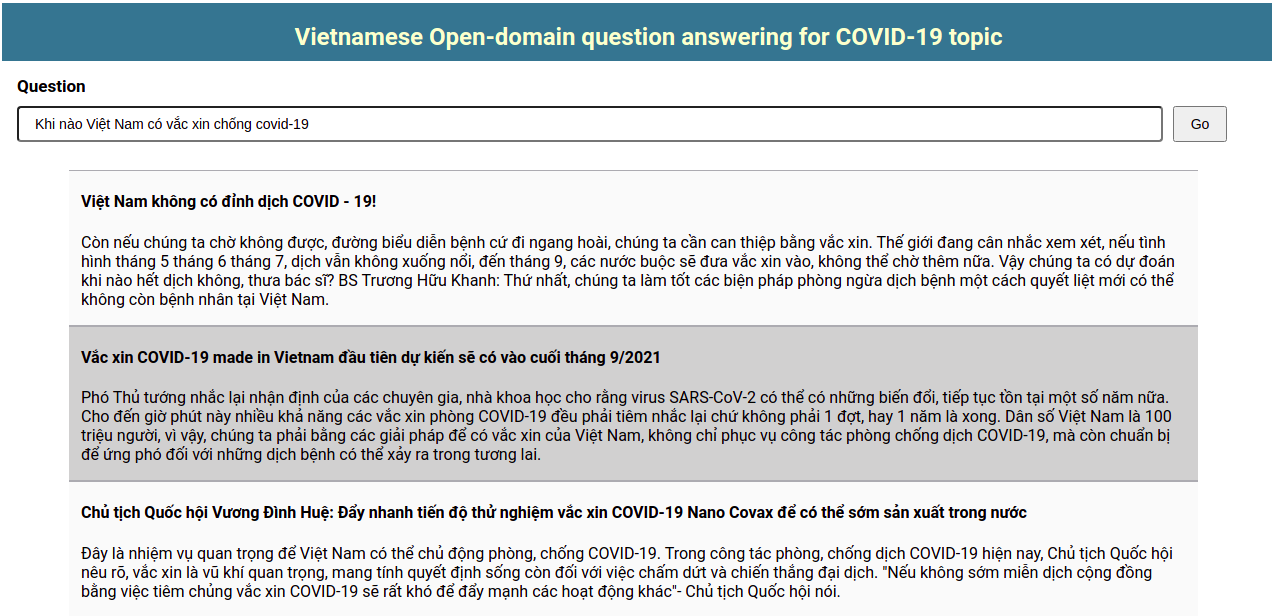
\includegraphics[scale=.27]{images/VNQA_2.png}
\end{adjustwidth}
\end{frame}
%=======================================
\section{Conclusion and future works}
\begin{frame}
\frametitle{Conclusion and future works}
\begin{center}
	\begin{itemize}
		\item Conclusion
		\begin{itemize}
			\item Propose to train retriever model with stratified loss
			\item Conduct a case study for open-domain question answering system in Vietnamese language for COVID-19 topic
			\item Use Cloud TPUs to train large retriever model in short time
		\end{itemize}
		\item Future works
		\begin{itemize}
			\item Study machine reading comprehension problem to improve reader component
			\item Study the relationship between open-domain question answering and automatic knowledge graph construction
			\item Study dialogue management problem, which extends question answering problem by adding multi-turn conversation ability
		\end{itemize}
	\end{itemize}
\end{center}
\end{frame}
%=======================================
\begin{frame}[plain]
	%\frametitle{Question Answering about COVID-19}
	\begin{center}
		\textcolor{blue}{\fontsize{20pt}{\baselineskip}\selectfont\bfseries Thank you for your attention}
	\end{center}
\end{frame}
\end{document}